\chapter{
تصویر تصادفی پایدار
}

روش تصویر تصادفی پایدار
\LTRfootnote{Stable Random Projections}
\cite{litez116, litez166, litez19, litez99, litez96, litez104}
یک روش پرکاربرد در داده‌کاوی و یادگیری ماشین است. با این روش به طور کار 
$l_\alpha (0 < \alpha \leq 2)$
فاصله در داده‌های حجیم (برای مثال: وب یا جریان‌های داده‌ی حجیم) محاسبه می‌شود. در این روش حافظه‌ی کمی استفاده شده و فقط یک بار پایش داده‌ها کافی است. 

\begin{figure}[h]
\centering
\begin{latin}
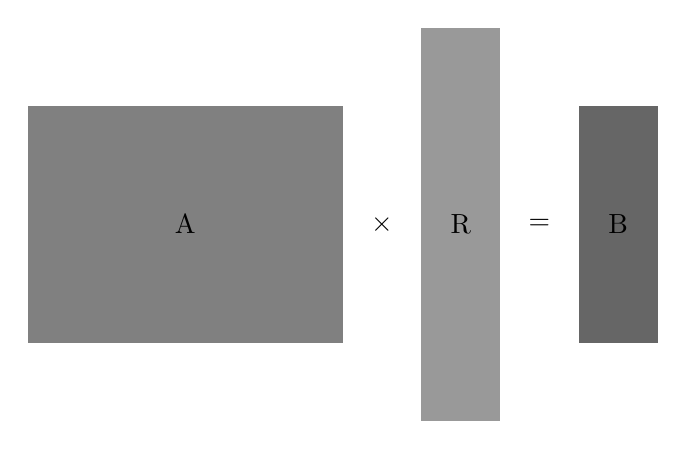
\begin{tikzpicture}
\fill[black!50!white] (0,1) rectangle (4,4);
\node at (2,2.5) [rectangle,preaction={fill=black!50},font={A}] {};
\node at (4.5,2.5) [rectangle,preaction={fill=black!0},font={$\times$}] {};
\fill[black!40!white] (5,0) rectangle (6,5);
\node at (5.5,2.5) [rectangle,preaction={fill=black!40},font={R}] {};
\node at (6.5,2.5) [rectangle,preaction={fill=black!0},font={=}] {};
\fill[black!60!white] (7,1) rectangle (8,4);
\node at (7.5,2.5) [rectangle,preaction={fill=black!60},font={B}] {};
\end{tikzpicture}
\end{latin}
\caption{
روش تصویر تصافی پایدار ماتریس داده‌ی 
$\mathbf{A} \in \mathbb{R}^{n \times D}$
را در یک ماتریس تصادفی
$\mathbf{R} \in \mathbb{R}^{D \times k}$
ضرب می‌کند تا ماتریس تصویر شده‌ی 
$\mathbf{B} = \mathbf{AR} \in \mathbb{R}^{n \times k}$
حاصل شود.
}
\label{fig:randomprojection}
\end{figure}

همانطور که در 
\autoref{fig:randomprojection}
می‌بینید. ایده تصویر تصادفی پایدار، ضرب ماتریس داده‌ها
$\mathbf{A} \in \mathbb{R}^{n \times D}$
در ماتریس تصادفی 
$\mathbf{R} \in \mathbb{R}^{D \times k}  (k \ll D)$
است که حاصل یک ماتریس تصویر شده‌ی 
$\mathbf{B} \in \mathbb{R}^{n \times k}$
است. درایه‌های ماتریس تصادفی 
$mathbf{R}$
به طور 
\lr{i.i.d.}
(مستقل و هم توزیع)
\LTRfootnote{Independent and Identically distributed}
از یک توزیع 
$\alpha$
-پایدار 
\LTRfootnote{$\alpha$-stable distribution}
حاصل می‌شوند. به همین دلیل به این روش «تصویر تصادفی پایدار» گفته می‌شود. به این نکته توجه کنید که توزیع 2-پایدار معادل توزیع نرمال و توزیع پایدار 1-پایدار معادل کوچی
\LTRfootnote{Cauchy}
است.

حالت خاص تصویر تصادفی نرمال (به عبارت دیگر
$\alpha = 2$
) نسبتا به خوبی مورد بررسی قرار گرفته است. به رساله
\cite{litez166}
مراجعه کنید. بنابراین، بخش اعظم این پایان‌نامه به تصویر تصادفی پایدار 
$\alpha < 2$
اختصاص یافته است.


پس از مروری بر حالت کلی تصویر تصادفی پایدار 
$0 < \alpha \leq 2$
، جزئیات بیشتری در خصوص حالت 
$l_2$
مورد بررسی قرار می‌گیرد. سپس ارتقاء روش با استفاده از اطلاعات حاشیه‌ای
\LTRfootnote{Marginal information}
بررسی می‌شود. در ادامه، تصویر تصادفی نرمال ساده‌سازی می‌شود. این کار با نمونه‌برداری 
$\mathbf{R}$
از حالت توزیع گسسته‌ی سه‌نقطه‌ای 
$[ -1, 0, 1]$
انجام می‌شود. این حالت، یک حالت خاص توزیع‌های زیرگوسی
\LTRfootnote{sub-Gaussian}
است. سپس نرم 
$l_1$
\LTRfootnote{Cauchy random projection}
مورد بررسی قرار گرفته و در ادامه حالت کلی 
$0 < \alpha \leq 2$
مورد بجث قرار می‌گیرد.

\section{
مسئله‌ی اصلی در تصویر تصادفی پایدار
}
مسئله اصلی تصویر تصادفی پایدار یک مسئله‌ی برآورد آماری است. همانطور که بیان شد، ماتریس داده‌ی 
$\mathbf{A} \in \mathbb{R}^{n \times D}$
را در ماتریس تصادفی 
$\mathbf{R} \in \mathbb{R}^{D \times k}$
ضرب می‌کنیم تا ماتریس بسیار کوچکتر 
$\mathbf{B} = \mathbf{A} \times \mathbf{R} \in \mathbb{R}^{n \times k}$
را بدست بیاوریم. هدف این است که مشخصات آماری 
$\mathbf{A}$
بر اساس ماتریس 
$\mathbf{B}$
استنتاج شوند. (شامل نرم و فاصله)

بدون از دست دادن کلیت، ما بر ۲ سطر اول 
$\mathbf{A}$
، 
$u_1, u_2 \in \mathbb{R}^D$
و دو سطر اول در 
$\mathbf{B}$
،
$v_1, v_2 \in \mathbb{R}^k$
تمرکز می‌کنیم. تعریف می‌کنیم
$ \mathbf{R} = \left \{ r_{ij} \right \}_{i=1}^D {}_{j=1}^{k}$
بنابراین:
\begin{align}
v_{1,j} = \sum_{i=1}^{D} r_{ij}u_{1,i},\;\;
v_{2,j} = \sum_{i=1}^{D} r_{ij}u_{2,i},\;\;
x_j = v_{1,j} - v_{2,j} = \sum_{i=1}^D r_{ij}(u_{1,i} - u_{2,i}).
\label{eq:1hm}
\end{align}

\subsection{
توزیع‌های پایدار
}

به طور معمول 
$r_{ij} \sim S(\alpha, 1)$
 و به طور 
\lr{i.i.d.}
استخراج می‌شود. همچنین در ادامه ما حالت‌های ساده‌تری را هم مورد بررسی قرار می‌دهیم. در اینجا 
$S(\alpha, 1)$
بیانگر یک توزیع متقارن 
$\alpha$
-پایدار تصادفی است
\cite{litez171}
با پارامتر اندیس 
$\alpha$
و پارامتر مقیاس ۱.

یک متغییر تصادفی 
$z$
در صورتی متقارن  
$\alpha$
-پایدار است که تابع مشخصه‌ی آن به شکل زیر باشد.

\begin{align}
E \big( \exp  \big( \sqrt{-1}zt \big)  \big) = \exp \big( -d |t|^\alpha \big)
\label{eq:1hn}
\end{align}

که 
$d>0$
پارامتر مقیاس است. ما می‌نویسیم 
$z \sim S(\alpha, d)$
که به طور کلی شکل بسته‌ای برای تابع چگالی ندارد. به جز حالت 
$\alpha = 2$
(نرمال) و 
$\alpha = 1$
(کوچی
\LTRfootnote{Cauchy}
).


\subsection{
مسئله برآورد آماری
}

با توجه به خواص تبدیل فوریه، به راحتی می‌توان نشان داد که داده‌های تصویر شده هم از توزیع 
$\alpha$
-پایدار پیروی می‌کنند که در این حالت پارامتر مقیاس مشخصه‌ی 
$l_\alpha$
ی (نرم‌ها، فاصله‌ها) داده‌های اصلی در 
$\mathbf{A}$
است. به طور خاص:
\begin{align}
v_{1,j} \sim S \bigg( \alpha, \sum_{i=1}^D |u_{1,i}|^\alpha \bigg), \;\;
v_{2,j} \sim S \bigg( \alpha, \sum_{i=1}^D |u_{2,i}|^\alpha \bigg),
 \label{eq:1hp}\\
x_j = v_{1,j} - v_{2,j} \sim S \bigg( \alpha, d_{(\alpha)} = 
\sum_{i=1}^D | u_{1,i} - u_{2,i} |^\alpha \bigg).
 \label{eq:1hq}
\end{align}
بنابراین، کار ما به برآورد پارامتر مقیاس از 
$k$
نمونه 
\lr{i.i.d.}
، 
$x_j \sim S \big( \alpha, d_{(\alpha)} \big)$
تقلیل پیدا می‌کند. به این خاطر که هیچ شکل بسته‌ای برای تابع چگالی به جز در حالت 
$\alpha = 1,2$
وجود ندارد، فرآیند تخمین خود مسئله‌ی جالبی است اگر به دنبال برآوردگرهایی بگردیم که هم به طور آماری دقیق باشند و هم از لحاظ محاسباتی کارا باشند.

یک موضوع مربوط و نزدیک هم تعیین اندازه نمونه
$k$
است. روش استاندارد محدود کردن احتمال دم است 
$\mathbf{Pr} \big( | \hat{d}_{(\alpha)} - d_{(\alpha)} | > \epsilon d_{(\alpha)} \big)$
که 
$\hat{d}_{(\alpha)}$
برآوردگری برای
$d_{(\alpha)}$
است و 
$\epsilon$
دقت مورد نظر است (معمولا 
$0<\epsilon<1$
). به طور ایده‌آل امیدوار هستیم نشان دهیم
\footnote{
بنابر قضیه حدمرکزی برآوردگر 
$\hat{d}_{(\alpha)}$
بر اساس
$k$
نمونه تحت شروط ساده‌ای به حالت نرمال همگرا می‌شود. بنابر محدوده‌ی دم نرمال می‌دانیم که حداقل برای پارامترهای خاصی 
$\mathbf{Pr} \big( | \hat{d}_{(\alpha)} - d_{(\alpha)} | \geq \epsilon d_{(\alpha)} \big) \leq 2 \exp \Big( -k \frac{\epsilon^2}{2V} \Big)$
باید صادق باشد. در اینجا 
$\frac{V}{k}$
واریانس مجانبی 
$\hat{d}_{(\alpha)}$
است. بنابراین، حداقل برای آزمون درستی، می‌توانیم با بررسی این‌که آیا
$\lim_{\epsilon \rightarrow 0+} G = 2V$
چک کنیم که محدوده‌ی دم نسبت مطلوب را دارا باشد.
}
:

\begin{align}
\mathbf{Pr} \big( | \hat{d}_{(\alpha)} - d_{(\alpha)}| > \epsilon d_{(\alpha)} \big) \leq 2 \exp \bigg( -k \frac{\epsilon^2}{G} \bigg),
\label{eq:1hr}
\end{align}

برای برخی مقادیر ثابت 
$G$
که می‌تواند تابعی از 
$\epsilon$
هم باشد.

برای ماتریس داده‌ی
$\mathbf{A} \in \mathbb{R}^{n \times D}$
، در مجموع 
$\frac{n(n-1)}{2} < \frac{n^2}{2}$
جفت فاصله وجود دارد. ما معمولا علاقمندیم که احتمالات دم را به طور همزمان برای همه‌ی جفت‌ها محدود کنیم. 

\section{
تصویر تصادفی نرمال
\label{SecNormal}
}
برای کاهش بعد در نرم 
$l_2$
، روش 
\textit{
تصویر تصادفی نرمال
}
ماتریس داده‌ی اولیه 
$\mathbf{A} \in \mathbb{R}^{n \times D}$
را در ماتریس تصادفی 
$\mathbf{R} \in \mathbb{R}^{D \times k} (k \ll D)$
با درایه‌های 
\lr{i.i.d.}
از 
$N(0,1)$
، تا ماتریس تصویر شده‌ی 
$\mathbf{B} \in \mathbb{R}^{n \times k}$
حاصل شود. تحلیل‌های مربوط به تصویر تصادفی نرمال نسبتا ساده است. برای مثال، به شکل سرراستی می‌توان یک نسخه از لم 
\lr{JL}
\LTRfootnote{Johnson-Lindenstrauss}
\cite{litez103}
را برای حالت 
$l_2$
استنتاج کرد.

ما در ابتدا برخی خواص اولیه تصویر تصادفی نرمال را بیان می‌کنیم و سپس بر روی اطلاعات حاشیه تمرکز می‌کنیم تا تخمین‌ها را بهینه کنیم. حاشیه‌ها (به عبارت دیگر، نرم 
$l_2$
برای هر خط در 
$\mathbf{A}$
)
معمولا در ابتدا در دسترس هستند (برای مثال، از طریق نرمال سازی داده‌ها). ولی حتی در حالتی که در دسترس نیستند، محاسبه‌ی نرم 
$l_2$
برای تمام سطرهای 
$\mathbf{A}$
فقط نیازمند یکبار مرور داده‌ها است که هزینه‌ای از 
$O(nD)$
دارد که قابل صرفنظر است.
\footnote{
این وضعیتی برای زمانی که با جریان داده‌های داینامیک سر و کار داریم اندکی متفاوت است. در جریان‌های داده ما معمولا به دنبال اطلاعات آماری یک جریان داده هستیم تا اختلاف میان دو جریان داده را مد نظر داشته باشیم. به عبارت دیگر، محاسبه نرم 
$l_2$
حاشیه‌ای گاهی اوقات هدف اصلی است. به دلیل ذات دینامیک جریان‌های داده (برای مثال، به روز شدن مدام)، محاسبه‌ی حاشیه‌ها می‌تواند پر هزینه باشد.
}
از آنجا که اعمال تصویر تصادفی 
$\mathbf{A} \times \mathbf{R}$
هم اکنون هزینه‌ای از مرتبه 
$O(nDk)$
دارد.

در این بخش، ما این قاعده مرسوم تبعیت در ادبیات تصویر تصادفی 
\cite{litez166}
پیروی می‌کنیم و تعریف می‌کنیم
$\mathbf{B} = \frac{1}{\sqrt{k}} \mathbf{A} \mathbf{R}$.

\subsection{
مشخصه‌های اصلی
}

ما فرض می‌کنیم یک ماتریس داده 
$\mathbf{A} \in \mathbb{R}^{n \times D}$
و یک ماتریس تصویرگر
$\mathbf{R} \in \mathbb{R}^{D \times k}$
که به طور 
\lr{i.i.d.}
از 
$N(0,1)$
تولید شده است. در نظر می‌گیریم
$\mathbf{B} = \frac{1}{\sqrt{k}} \mathbf{A} \mathbf{R}$
.
در نظر بگیرید
$u_i^T$
سطر
$i$
ام ماتریس 
$\mathbf{A}$
باشد، و سطر متناظر در 
$\mathbf{B}$
،
$v_i^T$
باشد.
برای راحتی بر روی دو سطر اول 
$\mathbf{A}$
یعنی 
$u_1$
و
$u_2$
همچنین دو سطر اولیه
$v_1$
و 
$v_2$
در 
$\mathbf{B}$
تمرکز می‌کنیم. تعریف می‌کنیم:

\begin{align}
a= u_1^T u_2, \; m_1 = \|u_1 \|^2, \; m_2 = \| u_2 \|^2, \; d =  \| u_1 - u_2 \|^2 = m_1 + m_2 - 2a
\label{eq:1i7}
\end{align}

به آسانی می‌توانیم نشان دهیم 
$\| v_1 - v_2 \|$
، فاصله‌ی 
$l_2$
نمونه و 
$v_1^T v_2$
ضرب داخلی نمونه، برآوردگرهای نااریبی از 
$d$
و 
$a$
هستند. لم ۱ واریانس و تابع مشخصه‌ی 
$v_1^T v_2$
را مشخص می‌‌کند. اثبات در 
\cite{li2007stable}
.

\textbf{لم ۱:}
$u_1, u_2 \in \mathbb{R}^D$
داده شده‌اند و یک ماتریس تصادفی
$\mathbf{R} \in \mathbb{R}^{D \times k}$
شامل درایه‌های 
\lr{i.i.d.}
از نرمال استاندارد
$N(0,1)$
. اگر مقادیر 
$v_1 = \frac{1}{\sqrt{k}} \mathbf{R}^T u_1$
و 
$v_2 = \frac{1}{\sqrt{k}} \mathbf{R}^T u_2$
را تعیین کنیم، داریم:

\begin{align}
E \big(  \| v_1 - v_2 \|^2 \big) = d, \;\;\; \mathit{Var}\big(\| v_1 - v_2 \|^2\big) = \frac{2}{k} d^2  \label{eq:1i8}\\
E \big( v_1^T v_2 \big) = a, \;\;\; \mathit{Var} \big(v_1^T v_2 \big) =  \frac{1}{k} \big(m_1 m_2 + a^2\big), \label{eq:1i9}
\end{align}

سومین ممان مرکزی 
$v_1^T v_2$
عبارت است از:

\begin{align}
E \big( v_1^T v_2 \big)^2 = a, \;\;\; \frac{2a}{k^2} \big( 2 m_1 m_2 + a^2 \big)
\label{eq:1iA}
\end{align}

و تابع مولد احتمال برای 
$v_1^T v_2$
عبارت است از:

\begin{align}
E \big( \exp \big( v_1^T v_2 t \big) \big)
 = \bigg(  1 - \frac{2}{k} at - \frac{1}{k^2} \big( m_1 m_2 - a^2 \big) t^2 \bigg)^{- \frac{k}{2}}
\label{eq:1iB}
\end{align}

که 
$\frac{-k}{\sqrt{m_1 m_2} - a} \leq t \leq \frac{-k}{\sqrt{m_1 m_2} + a}$
است.

بنابراین، برآوردگرهای نااریبی برای فاصله 
$l_2$
$d$
و ضرب داخلی
$a$
به شکل سر راستی عبارت است از:

\begin{align}
\hat{d}_{MF} = \| v_1 - v_2 \|^2, \;\;\; \mathit{Var} \Big( \hat{d}_{MF} \Big) = \frac{d^2}{k}, \label{eq:1iC}\\
\hat{a}_{MF} = v_1^T v_2, \;\;\; \mathit{Var} \big( \hat{a}_{MF} \big) = \frac{1}{k} \big( m_1 m_2 + a^2 \big), \label{eq:1iD}
\end{align}

که اندیس «
$MF$
» به معنی «بدون حاشیه»
\LTRfootnote{margin-free}
نشان دهنده این است که برآوردگرها از اطلاعات حاشیه‌ای 
$m_1 = \| u_1 \|^2$
و 
$m_2 = \| u_2 \|^2$
استفاده نمی‌کنند.

به این نکته توجه کنید که، 
$k \hat{d}_{MF} / d$
از توزیع 
$\chi^2$
با 
$k$
درجه آزادی، پیروی می‌کند،
$\chi_k^2$
. بنابراین، به راحتی می‌توان می‌توانیم این محدوده‌‌های دم را برای لم ۲ اثبات کنیم.

\textbf{
لم ۲:
}

\begin{align}
\mathbf{Pr} \big( \hat{d}_{MF} - d > \epsilon d) \leq \exp \Bigg( - \frac{k}{2} \big( \epsilon - \log( 1+ \epsilon) \big) \Bigg), \;\;\; \epsilon > 0 
\label{eq:1iE} \\
\mathbf{Pr} \big( \hat{d}_{MF} - d < -\epsilon d) \leq \exp \Bigg( - \frac{k}{2} \big( -\epsilon - \log( 1 - \epsilon) \big) \Bigg), \;\;\; 0 < \epsilon < 1 
\label{eq:1iF} 
\end{align}

\textbf{
اثبات:
}

از آنجا که 
$k \hat{d}_{MF} / d \sim \chi_k^2 $
، بر اساس نام مساوی چرنوف
\LTRfootnote{Chernoff inequality}
\cite{litez46}
، برای هر 
$t > 0$ 
داریم:

\begin{align}
\begin{split}
\mathbf{Pr} \big( \hat{d}_{MF} - d > \epsilon d) = 
\mathbf{Pr} \big( k \hat{d}_{MF} / d > k(1+\epsilon) \big) \\
\leq 
\frac{E\bigg( \exp (k \hat{d}_{MF} /dt \bigg) }{\exp \big( (1+\epsilon ) kt \big) } =
\exp \Bigg( - \frac{k}{2} \big( \log (1-2t) + 2(1 + \epsilon) t \big) \Bigg)
\end{split}
\label{eq:1iG}
\end{align}

که در 
$t = t_{NR} = \frac{\epsilon}{2(1+\epsilon)}$
و بنابراین برای هر 
$\epsilon > 0$
داریم:

\begin{align}
\mathbf{Pr} \big( \hat{d}_{MF} - d > \epsilon d) \leq \exp \left( -\frac{k}{2} \left( \epsilon - \log \left( 1 + \epsilon \right) \right) \right)
\label{eq:1iH}
\end{align}

ما می‌توانیم به طور مشابه برای دیگر محدوده‌ی دم 
$\mathbf{Pr} \big( \hat{d}_{MF} - d < -\epsilon d)$
هم اثبات کنیم.
$\blacksquare$

\bigskip

برای راحتی مرسوم است که محدوده دم را در لم ۲ به صورت متقارن 
$\mathbf{Pr} \left( \left| \hat{d}_{MF} - d \right| > \epsilon d \right)$
نوشته شود. نامساوی‌های ساده‌ای برای 
$\log(1+\epsilon)$
و 
$\log(1-\epsilon)$
نتیجه می‌دهد:

\begin{align}
\mathbf{Pr} \left( \left| \hat{d}_{MF} - d \right| \geq \epsilon d \right) \leq 2 \exp \left( - \frac{k}{4} \epsilon^2 + \frac{k}{6} \epsilon^3 \right),\;\; 0 < \epsilon < 1
\label{eq:1iI}
\end{align}

از آنجا که 
$\mathbf{A} \in \mathbb{R}^{n \times D}$
تعداد 
$n$ 
سطر دارد. به عبارت دیگر 
$\frac{n(n-1)}{2}$
جفت. ما باید احتمال دم را به طور همزمان برای همه‌ی جفت‌ها محدود کنیم. با استفاده از محدوده تجمیعی بنفرونی
\LTRfootnote{Benferroni union bound}
کافی است که:

\begin{align}
\frac{n^2}{2} \mathbf{Pr} \left( \left| \hat{d}_{MF} - d \right| \geq \epsilon d \right) \leq \delta
\label{eq:1iJ}
\end{align}

به عبارت دیگر کافی است اگر:

\begin{align}
\frac{n^2}{2} 2 \exp \left( - \frac{k}{4} \epsilon^2 + \frac{k}{6} \epsilon^3 \right) \leq \delta 
\Rightarrow
k \geq \frac{2 \log n - \log \delta}{\epsilon^2 / 4 - \epsilon^3 / 6}
\label{eq:1iK}
\end{align}

بنابراین ما یک نسخه‌ای از لم 
\lr{JL}
را نشان داده‌ایم.

\textbf{
لم ۳:
}
اگر 
$k \geq \frac{2 \log n - \log \delta}{\epsilon^2 / 4 - \epsilon^3 / 6} $
پس با حداقل احتمال 
$1-\delta$
، فاصله 
$l_2$
بین هر جفت از داده‌ها (میان 
$n$
نقطه) می‌تواند با ضریب اطمینان
$1 \pm \epsilon$
با استفاده فاصله‌ی 
$l_2$
در داده‌های تصویر شده بعد از تصویر تصافی نرمال، تخمین زده شود.
$0 < \delta < 1, 0 < \epsilon < 1$
.
$\blacksquare$
\bigskip


%===============================================================================S

\section{
تصویر تصادفی زیر گوسی و بسیار پراکنده
}

در بخش قبل ما به بررسی تصویر تصادفی نرمال پرداختیم، که در آن ماتریس تصویرگر 
$\mathbf{R}$
از روی توزیع 
$N(0,1)$
به طور 
\lr{i.i.d.}
نمونه‌گیری می‌شود. این انتخاب خاص برای 
$\mathbf{R}$
، صرفا برای سهولت تحلیل تئوری است. در واقع می‌توان 
$\mathbf{R}$
را از هر توزیعی با میانگین صفر و واریانس محدود برای کاهش بعد در نرم 
$l_2$
نمونه‌گیری کرد.

نمونه‌گیری
$\mathbf{R}$
از یک توزیع زیرگوسی
\LTRfootnote{sub-Gaussian}
هم از نظر تئوری قابل قبول و هم از جنبه‌ی محاسباتی تسهیل کننده است. برای مثال، محدوده‌ی دم زیر گوسی به سادگی به نسخه‌ای از لم
\lr{JL}
منتهی می‌شود. 

ما بر روی یک انتخاب معمول از توزیع زیر گوسی تمرکز خواهیم کرد، که درایه‌ها ماتریس 
$\mathbf{R}$
از مجموعه‌ی 
$\left\{ -1, 0, 1 \right\}$
با احتمالات 
$\left\{ \frac{1}{2s}, 1 - \frac{1}{s}, \frac{1}{2s} \right\}$
، که 
$s \geq 1$
. به این ترتیب فرآیند نمونه‌گیری ساده‌تر شده و محاسبات سریعتر انجام می‌شوند. در واقع، زمانی که 
$s < 3$
باشد، واریانس‌های صرحا کوچکتری نسبت به استفاده از تصویر تصادفی نرمال بدست می‌آید.

با در نظر گرفتن قواعد معقول، برای مثال، داده‌های اولیه ممان سوم محدود داشته باشند،می‌توانیم 
$s \gg 3$
در نظر بگیریم (حتی 
$s = \sqrt{D}$
).
تا نتایج 
$s$
برابر سریعتر بدست بیاوریم؛ و بنابراین، این رویه را تصویر تصادفی بسیار پراکنده می‌نامیم.

%============================================================================================A

\subsection{
تصویر تصادفی زیرگوسی
}

مشابه
\autoref{SecNormal}
ماتریس داده را 
$\mathbf{A} \in \mathbb{R}^{n \times D}$
در نظر می‌گیریم. ماتریس تصویر تصادفی 
$\mathbf{R} \in \mathbb{R}^{D \times k}$
را تولید کرده و آن را در 
$\mathbf{A}$
ضرب می‌کنیم تا به یک ماتریس تصویر شده‌‌ی 
$\mathbf{B} = \frac{1}{\sqrt{k}} \mathbf{AR} \in \mathbb{R}^{n \times k}$
برسیم. دوباره رو دو ردیف ابتدایی تمرکز می‌کنیم، که یعنی 
$u_1$
و 
$u_2$
در 
$\mathbf{A}$
، و دو ردیف ابتدایی 
$v_1$
و 
$v_2$
در 
$\mathbf{B}$
و همچنین تساوی‌های زیر را تعریف می‌کنیم:

\begin{align}
a = u_1^T u_2, \;\;\; m_1 = \| u_1 \|^2, \;\;\; m_2 = \| u_2 \|^2, \;\;\;
d = \| u_1 - u_2 \|^2 = m_1 + m_2 - 2a
\label{eq:1iL}
\end{align}

$\mathbf{R}$
را به طور 
\lr{i.i.d}
از یک توزیع زیر گوسی مشخصا پرکاربرد تولید می‌کنیم:(
$S \geq 1$
)

\begin{align}
r_{ij} = \sqrt{s} \times 
\begin{cases}
1 & \text{با احتمال} \;\; \frac{1}{2s}\\
0 & \text{با احتمال} \;\; 
1-\frac{1}{s}\\
-1 & \text{با احتمال} \;\; \frac{1}{2s}
\end{cases} 
\label{eq:1iM}
\end{align}

\begin{itemize}
\item
نمونه‌گیری از 
\autoref{eq:1iM}
ساده‌تر از نمونه‌گیری از
$N(0,1)$
است.
\item
می‌تواند از 
$s$
برابر افزایش سرعت در ضرب ماتریسی 
$\mathbf{A} \times \mathbf{R}$
بهره برد، زیرا فقط
$\frac{1}{s}$
داده‌های نیازمند پردازش هستند.
\item
نیازی به عملیات محاسباتی با ممیز شناور نیست و تمامی بار محاسباتی بر روی عملیات تجمیع پایگاه داده است که به خوبی بهینه شده.
\item
وقتی 
$s<3$
باشد می‌توان به تخمین‌هایی با دقت بیشتر (واریانس کمتر) دست پیدا کرد.
\item
هزینه نگهداری ماتریس 
$\mathbf{R}$
از 
$O(Dk)$
به 
$O(Dk/s)$
کاهش می‌یابد.
\end{itemize}

\cite{litez2, litez3}
نشان ‌می‌دهند زمانی که 
$s=1$
و 
$s=3$
باشد، می‌توان به همان محدوده‌ی 
\lr{JL}
ای دست پیدا کرد که در تصویر تصادفی نرمال وجود دارد. ما در ادامه به بررسی خواص توزیع زیر گوسی می‌پردازیم، که برای تحلیل محدوده‌ی دم مناسب است. در واقع، آنالیز زیر گوسی نشان می‌دهد که می‌توان حتی در بدترین شرایط از مقادیری اندکی بیشتر از ۳ برای 
$s$
استفاده کرد.

\subsubsection{
توزیع زیر گوسی
}

ما در اینجا مقدمه‌ای کوتاه بر توزیع‌های زیرگوسی بیان می‌کنیم. برای جزئیات و منابع بیشتر می‌توانید به
\cite{litez40}
مراجعه کنید. تئوری توزیع‌های زیرگوسی در حدود 1960 آغاز شد.

متغییر تصادفی 
$x$
زیرگوسی است اگر ثابت 
$g > 0$
وجود داشته باشد به شکلی که:

\begin{align}
\mathrm{E}(\exp (xt)) \leq \exp \left( \frac{g^2 t^2}{2} \right), \forall t \in \mathbb{R}
\label{eq:1iN}
\end{align}

می‌توان مقدار بهینه‌ی 
$g^2$ 
را از تعریف 
$T^2(x)$
با استفاده از فرمول زیر بدست آورد.

\begin{align}
T^2(x) = \sup_{t \neq 0} \frac{2 \log \mathrm{E}\left(\exp(xt)\right)}{t^2}
\label{eq:1iP}
\end{align}

توجه کنید که 
$T^2(x)$
فقط یک نمادگذاری برای مقدار ثابت بهینه‌ی زیرگوسی یک متغییر تصادفی 
$x$
است (و نه یک نمونه مشخص از 
$x$
).

برخی از ویژگی‌های اولیه‌ی توزیع‌های زیرگوسی:

\begin{itemize}
\item
اگر 
$x$
زیر گوسی باشد آنگاه 
$\mathrm{E}(x) = 0$
و 
$\mathrm{E}(x^2) \leq T^2(x)$
. برای هر مقدار ثابت 
$c$
، 
$T^2(cx) = c^2T^2(x)$
. و
\begin{align}
\mathbf{Pr}(|x| > t) \leq 2 \exp \left( - \frac{t^2}{2T^2(x)} \right)
\label{eq:1iQ}
\end{align}
\item
اگر 
$x_1, x_2, \ldots, x_D$
زیرگوسی مستقل باشند، آنگاه
$\sum_{i=1}^D x_i$
زیرگوسی است.

\begin{align}
T^2 \left( \sum_{i=1}^D x_i \right) \leq \sum_{i=1}^D T^2(x_i)
\label{eq:1iR}
\end{align}
\item
اگر 
$x$
زیرگوسی باشد، آنگاه برای همه‌ی 
$t \in [0,1)$
،
\begin{align}
\mathbf{E} \left( \exp \left( \frac{x^2 t}{2 T^2(x)} \right) \right) \leq (1-t)^{- \frac{1}{2}}
\label{eq:1iS}
\end{align}

\cite{litez2, litez3}
همچنین 
\autoref{eq:1iS}
را برای توزیع ویژه‌ی
\autoref{eq:1iM}
بدست آورده‌اند. یک متغییر تصادفی زیرگوسی
$x$
صریحا زیرگوسی است اگر 
$\mathrm{E}(x^2) = T^2(x)$
\item
اگر 
$x$
صریحا زیر گوسی باشد، آنگاه 
‌$\mathrm{E}(x^3)=0$
و کشیدگی
\LTRfootnote{kurtosis}
غیر مثبت خواهد بود، به عبارت دیگر 
$\frac{\mathrm{E}(x^4)}{\mathrm{E}^2(x^2)} - 3 \leq 0$
.
\item
اگر
$x_1, x_2, \ldots, x_D$
صریحا زیرگوسی مستقل باشند، آنگاه
$\sum_{i=1}^D x_i$
صریحا زیرگوسی است.

\begin{align}
T^2 \left( \sum_{i=1}^D x_i \right) = \sum_{i=1}^D T^2(x_i)
= \sum_{i=1}^D \mathbf{E} \left( x_i^2 \right)
\label{eq:1iR}
\end{align}
\end{itemize}

$\blacksquare$
\bigskip


%=============================================================================A
\section{
تصویر تصادفی کوچی برای 
$l_1$
}
در بخش‌های قبلی به تصویر تصادفی برای کاهش بعد در نرم 
$l_2$
پرداخته شد. در این بخش به کاهش بعد در نرم
$l_1$
پرداخته خواهد شد. 

در اینجا هم با یک ماتریس داده‌ی 
$\mathbf{A} \in \mathbb{R}^{n \times D}$
کار خواهیم کرد. و یک ماتریس تصویرگر تصادفی 
$\mathbf{R} \in \mathbb{R}^{D \times k}$
که به طور 
\lr{i.i.d.}
از توزیع کوچی استاندارد 
$C(0,1)$
نمونه‌گیری شده است، تولید خواهیم کرد.
ما اجازه خواهیم داد که ماتریس تصویرشده 
$\mathbf{B} = \mathbf{A} \times \mathbf{R} \in \mathbb{R}^{n \times k}$
باشد. بدون آنکه ضریب نرمال‌سازی 
$\frac{1}{\sqrt{k}}$
که در بخش‌های قبلی مشاهده کردیم، حضور داشته باشد. ضمن آنکه این کار به یک تخمین آماری منجر خواهد شد که پارامتر مقیاس‌دهی را از تعداد 
$k$
متغییر تصادفی کوچی به طور 
\lr{i.i.d.}
برآورد می‌کند.

از آنجا که کوچی میانگین محدود ندارد. نمی‌توانیم از یک برآوردگر خطی آنطور که در تصویر تصادفی نرمال استفاده کردیم، استفاده کنیم. علاوه بر این، نتیجه‌ی عدم امکان بیان شده در 
\cite{litez32, litez109, litez33}
اثبات کرده است که وقتی از یک تصویرگر خطی استفاده شود، نمی‌توان از برآوردگرهای خطی بدون رخ دادن خطاهای بزرگ استفاده کرد. به عبارت دیگر، لم
\lr{JL}
برای 
$l_1$
صدق نمی‌کند.

در این بخش سه برآوردگر غیرخطی ارائه و یک معادل برای لم 
\lr{JL}
برای 
$l_1$
استنتاج  می‌شود. از آنجا که برآوردگرهای ما، متریک نیستند، این معادل لم 
\lr{JL}
از حالت کلاسیک لم
\lr{JL}
برای 
$l_2$
ضعیفتر است.

%============================================================================A
\subsection{
خلاصه نتایج اصلی
}

ما دوباره مانند بخش‌های قبلی دو سطر اول 
$A$
،
$u_1$
و 
$u_2$
و دو سطر اول 
$B$
،
$v_1$
و 
$v_2$
را در نظر می‌گیریم. فاصله‌ی 
$l_1$
را با 
$d = \sum_{i=1}^D | u_{1,i} - u_{2,i} | $
تعریف می‌کنیم. 

در تصویر تصادفی کوچی، فعالیت اصلی آن است که پارامتر مقیاس‌دهی کوچی از 
$k$
نمونه‌ی 
$x_j \sim C(0,d)$
به طور 
\lr{i.i.d.}
استخراج شود. برخلاف تصویر تصادفی نرمال، نمی‌توان 
$d$ 
را از میانگین نمونه برآورد کرد (به عبارت دیگر، 
$\frac{1}{k} \sum_{j=1}^k \left| x_j \right|$
زیرا 
$\mathrm{E}(x_j) = \infty$
. 

سه نوع برآوردگر غیر خطی مورد بررسی قرار خواهند گرفت: برآوردگرهای میانه‌ی نمونه، برآوردگرهای میانگین هندسی و برآوردگرهای حداکثر درستنمایی.

\begin{itemize}
\item
\textbf{
برآوردگرهای میانه نمونه
}

برآوردگر‌ میانه‌ی نمونه 
$\hat{d}_{me}$
و نسخه‌ی بدون انحراف 
$\hat{d}_{me,c}$
به شکل زیر هستند.

\begin{align}
\hat{d}_{me} = \mathrm{median} \left( \left| x_j \right|, j=1,2, \ldots, k \right)\\
\hat{d}_{me,c} = \frac{\hat{d}_{me}}{b_{me}}\\
b_{me} = \int_0^1 \frac{(2m+1)!}{(m!)^2} \tan \left( \frac{\pi}{2} t \right) \left( t - t^2 \right)^2 dt, \;\;\; k = 2m+1
\label{eq:1iT}
\end{align}

برای سهولت، ما فقط 
$k = 2m+1, m = 1,2, \ldots$
را در نظر می‌گیریم.

در بین تمامی برآوردگرهای چندکی، 
$\hat{d}_{me}$
(و 
$\hat{d}_{me,c}$
) کوچکترین مقدار واریانس مجانبی را بدست می‌دهد.

\item
\textbf{
برآوردگرهای میانگین هندسی
}

برآوردگر میانگین هندسی، 
$\hat{d}_{gm}$
و نسخه‌ی بدون انحراف 
$\hat{d}_{gm,c}$
به شکل زیر هستند:

\begin{align}
\hat{d}_{gm} = \prod_{j=1}^k \left| x_j \right|^{1/k}\\
\hat{d}_{gm,c} = \cos^k \left( \frac{\pi}{2k} \right) \prod_{j=1}^k \left| x_j \right|^{1/k}
\label{eq:1iU}
\end{align}

از نظر واریانس‌های مجانبی، برآوردگرهای میانگین هندسی به صورت مجانبی متناظر با برآوردگرهای میانه‌ی نمونه هستند. اگر چه از نظر محدوده‌ی دم، برآوردگرهای میانه‌ی نمونه ممکن است نیازمند نمونه‌ای به اندازه‌ی تا دو برابر بزرگتر باشند.

\item
\textbf{
برآوردگر حداکثر درستنمایی
}

این برآوردگر که به صورت 
$\hat{d}_{MLE,c}$
تعریف می‌شود. برآوردگر بدون انحراف حداکثر درستمانی (
\lr{MLE}
) عبارت است از:

\begin{align}
\hat{d}_{MLE,c} = \hat{d}_{MLE} \left( 1 - \frac{1}{k} \right)
\label{eq:1iU}
\end{align}

که 
$\hat{d}_{MLE}$
یک معادله‌ی غیر خطی 
\lr{MLE}
را حل می‌کند.

\begin{align}
- \frac{k}{\hat{d}_{MLE}} + \sum_{j=1}^k \frac{2\hat{d}_{MLE}}{x_j^2 + \hat{d}_{MLE}^2 } = 0
\label{eq:1iV}
\end{align}

برآوردگرهای میانه‌ی نمونه و میانگین هندسی از نظر واریانس مجانبی، دقتی معادل 
$80\%$
\lr{MLE}
دارند. در حالی که استنتاج محدوده‌های دمی فرم-بسته دشوار است. نشان‌ خواهیم داد که توزیع 
$\hat{d}_{MLE,c}$
را می‌توان به وسیله‌ی یک معکوس گوسی
\LTRfootnote{Inverse Gaussian}
تخمین زد.

\end{itemize}



%=============================================================================A
\section{
تصویر تصادفی 
$\alpha$
-پایدار
}
توضیحات
در بخش‌های قبلی، در مورد تصویر تصادفی نرم 
$l_2$
و تصویر تصادفی نرم
$l_1$
صحبت کردیم. در این بخش، کاهش بعد در نرم 
$l_\alpha$
، برای 
$0 < \alpha \leq 2$
مورد بررسی قرار خواهد گرفت. و نرم‌های 
$l_1$
و 
$l_2$
به عنوان حالت خاص بررسی می‌شوند.

مسئله اساسی در تصویر تصادفی پایدار، انجام برآورد آماری است. به عبارت دیگر، برآورد پارامتر مقیاس‌دهی توزیع پایدار متقارن. از آنجا که  چگالی احتمال توزیع پایدار جز برای 
$\alpha = 1, 2$
فرم بسته‌ ندارد. تولید برآوردگرهایی که از نظر آماری دقیق و از نظر محاسباتی بهینه هستند، جذاب است.

برآوردگرهایی که بر اساس میانه‌های نمونه (با به طور کلی بر اساس چندک‌های نمونه) تولید شده‌اند، در علم آمار شناخته‌شده‌اند، اما خیلی دقیق نیستند به خصوص در مورد نمونه‌های کوچک، و برای تحلیل نظری از جمله محدوده‌های دم زمانی که 
$\alpha \neq 1, 2$
راحت نیستند. 

ما در اینجا برآوردگر‌های مختلفی را بر اساس میانگین هندسی، میانگین هارمونیک
\LTRfootnote{Harmonic mean}
 و توان نسبی 
\LTRfootnote{Fractional power}
بررسی خواهیم کرد.


\subsection{
نتایج اصلی
}
گفته شد که، اگر دو بردار 
$u_1, u_2 \in \mathbb{R}^D$
(برای مثال،
$u_1$
و 
$u_2$
دو ردیف اول در ماتریس داده‌ی 
$\mathbf{A}$
باشند)
، اگر 
$v_1 = \mathbf{R}^T u_1$
و 
$v_2 = \mathbf{R}^T u_2$
باشند که 
$\mathbf{R} = \mathbb{R}^{D \times k}$
شامل نمونه‌های 
\lr{i.i.d.}
در 
$S(\alpha, 1)$
باشد، آنگاه 
$x_j = v_{1,j} - v_{2,j}, j = 1,2, \ldots, k$
، همگی
$S(\alpha, d_{(\alpha)})$
های 
\lr{i.i.d.}
هستند. که
$d_{(\alpha)} = \sum_{i=1}^D \left| u_{1,i} - u_{2,i} \right|^{\alpha}$.
بنابراین مسئله اصلی برآورد پارامتر مقیاس‌دهی 
$d_{(\alpha)}$
از تعداد 
$k$
نمونه‌ی 
\lr{i.i.d.}
توزیع
$S(\alpha, d_{(\alpha)}$
است. 
در بخش‌های قبلی به طور خلاصله توزیع‌های پایدار را مرور کردیم.

برآوردگری پرکاربرد در آمار بر اساس نمونه میان چندکی 
\LTRfootnote{inter-quantiles}
\cite{litez67, litez68, litez138}
است  که به دلیل تقارن 
$S(\alpha, d_{(\alpha)}$
می‌توان آن را به صورت برآوردگر میانه‌ی نمونه، ساده‌سازی کرد.

\begin{align}
\hat{d}_{(\alpha),me} = \frac
{ \mathrm{median} \left \{ \left| x_j \right|^{\alpha} , j = 1,2, \ldots, k \right \} }
{ \mathrm{median} \left \{ S(\alpha, 1) \right \}^{\alpha} }
\label{eq:1iW}
\end{align}

علی‌رغم سادگی، مسائل بسیاری براساس برآوردگر میانه‌ی نمونه
$\hat{d}_{(\alpha), me}$
وجود دارند. این برآوردگر، علی الخصوص برای نمونه‌های کوچک یا 
$\alpha$
ی کوچک دقیق نیست. همچنین برای تحلیل نظری دقیق از جمله تحلیل محدوده‌ی دم دشوار است.

ما برآوردگرهای زیادی را بر اساس میانگین هندسی، میانگین هارمونیک و توان کسری ارائه خواهیم کرد.

\begin{itemize}
\item
برآوردگر میانگین هندسی (بدون انحراف) 
$\hat{d}_{(\alpha),gm}$
:
\item
برآوردگر میانگین هندسی (دارای انحراف) 
$\hat{d}_{(\alpha),gm,b}$
:

این معادله به طور مجانبی معادل
$\hat{d}_{(\alpha),gm}$
است. اگرچه برای 
$0.25 \leq \alpha \leq 1$
، توزیع
$\hat{d}_{(\alpha),gm,b}$
خطای میانگین مربعات کوچکتری در مقایسه با
$\hat{d}_{(\alpha),gm}$
دارد.
\item
برآوردگر میانگین هارمونیک 
$\hat{d}_{(\alpha),hm}$
:
این معادله زمانی که 
$\alpha \rightarrow 0+$
به صورت مجانبی بهینه است و در مقایسه با برآوردگرهای میانگین هندسی، برای 
$\alpha \leq 0.344$
واریانس مجانبی کوچکتری دارد.

\item
برآوردگر میانگین ریاضی

برای 
$\alpha = 2$
بهترین روش استفاده از برآوردگر میانگین ریاضی 
$\frac{1}{k} \sum_{j=1}^k \left| x_j \right|^2$
است. این برآوردگر را می‌توان با استفاده از برآوردگر بیشینه درستنمایی، به شکلی که در بخش تصویر تصادفی نرمال توضیح داده شد، با استفاده از اطلاعات حاشیه‌آی ارتقاع داد.
\item
برآوردگر توان کسری
$\hat{d}_{(\alpha),fp}$
:

برای 
$\alpha = 2, \hat{d}_{(\alpha), fp}$
معادل برآوردگر میانگین ریاضی و برای 
$\alpha \rightarrow 0+$
معدل برآوردگر میانگین هارمونیک است. علاوه بر این، برای 
$\alpha \rightarrow 1$
،
$\hat{d}_{(\alpha),fp}$
دارای واریانس مجانبی برابر با برآوردگر میانگین هندسی است.
\end{itemize}

$\blacksquare$
\bigskip




%=============================================================================A
\chapter{
کاهش بعد و نحوه‌ی بررسی عملکرد آن
}
توضیحات

\section{
\lr{PCA}
و مقایسه با آن
}
توضیحات
\section{
برآوردگر‌ای معیارهای وابستگی
}
توضیحات
\section{
داده‌های مورد استفاده
}
توضیحات
\section{
توضیحات کد
}
توضیحات
\section{
شاخص محاسبه عملکرد کاهش بعد و 
\lr{Adjusted Rand Index}
}


\chapter{
نتایج
}




















